\newpage

\section{Программная реализация}
В данном разделе будут рассмотрены средства, методы и библиотеки, которые использовались при программной реализации. Кроме того, тут будут описаны основные функции, которые реализованы в модулях, и то как они работают. Так же будет рассмотрен процесс работы системы на заданном примере. 

Для наглядного описания взаимодействия разработанных компонентов ниже приведена диаграмма вариантов использования (рисунок~\ref{f:diag-comp}).

\begin{figure}[h!]
    \centering
    \vspace{\toppaddingoffigure}
    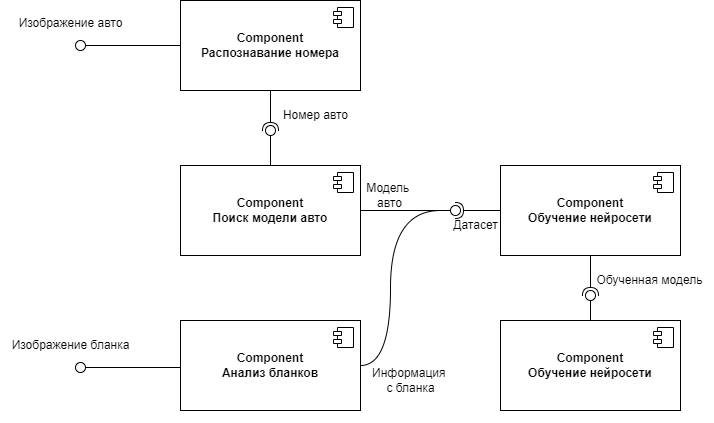
\includegraphics[width=0.8\textwidth]{diag-comp}
    \caption{Диаграмма компонентов}
    \label{f:diag-comp}
\end{figure}

\subsection{Программная реализация модуля для сбора данных}

В данном разделе рассматриваются технологии, используемые при реализации, и описывается сама программная реализация всех компонентов, которые выходят в модуль сбора данных.

\subsubsection{Анализ бланков}

В коде компонента используются библиотеки «cv2» (OpenCV) для обработки изображений, «numpy» для работы с массивами, «argparse» для обработки аргументов командной строки, «imutils» для удобных функций обработки изображений, «csv» для записи результатов в CSV-файл и «pytesseract» для распознавания текста на изображении.
Сам компонент имеет следующие основные функции:

\begin{enumerate}
    \item process\_exam(image\_path). Функция принимает путь к изображению листа. Используя библиотеку «cv2», выполняет следующие шаги обработки изображения:
        \begin{enumerate}
            \item преобразует изображение в оттенки серого, размывает его и применяет пороговое преобразование для выделения контуров;
            \item находит контуры на изображении и выбирает наибольший контур, который предположительно является контуром экзаменационного листа;
            \item используя функцию «four\_point\_transform» из «imutils», выполняет перспективное преобразование изображения, чтобы получить прямоугольный экзаменационный лист;
            \item применяет пороговое преобразование к преобразованному изображению и находит контуры вопросов на экзаменационном листе;
            \item для каждого вопроса находит наибольший контур, который предположительно является контуром выбранного ответа;
            \item определяет выбранные ответы и возвращает результаты в виде списка;
        \end{enumerate}
    \item get\_age(image\_path). Функция принимает путь к изображению документа, содержащего возраст. Используя библиотеку «cv2», выполняет следующие шаги обработки изображения:
        \begin{enumerate}
            \item находит контуры на изображении и выбирает наибольший контур, который предположительно является контуром документа;
            \item используя функцию «four\_point\_transform» из «imutils», выполняет перспективное преобразование изображения, чтобы получить прямоугольный документ;
            \item применяет пороговое преобразование к преобразованному изображению и находит контуры чисел на документе;
            \item используя библиотеку «pytesseract», выполняет распознавание текста на изображении и находит числа, представляющие возраст;
            \item возвращает возраст в виде строки;
        \end{enumerate}
    \item write\_to\_csv(filename, results):
        \begin{enumerate}
            \item функция принимает путь к CSV-файлу и результаты обработки;
            \item используя библиотеку «csv», открывает файл в режиме добавления и записывает результаты в виде строки в CSV-файл;
        \end{enumerate}
    \item blank(path\_in, path\_out, model):
        \begin{enumerate}
            \item функция принимает путь к входному изображению, путь к выходному CSV-файлу и модель (номер экзаменационного листа);
            \item вызывает функции «process\_exam» и «get\_age» для обработки изображения и определения возраста;
            \item добавляет модель и возраст в начало списка результатов;
            \item вызывает функцию «write\_to\_csv» для записи результатов в CSV-файл;
        \end{enumerate}
    \item main():
        \begin{enumerate}
            \item основная функция, которая принимает путь к входному изображению и путь к выходному CSV-файлу с помощью аргументов командной строки;
            \item вызывает функции «process\_exam» и «get\_age» для обработки изображения и определения возраста;
            \item вызывает функцию «write\_to\_csv» для записи результатов в CSV-файл;
        \end{enumerate}
\end{enumerate}

\subsubsection{Поиск модели авто}

При программной реализации данного компонента использовалась библиотеку Selenium для автоматизации веб-браузера. Она включает в себя следующие функции и шаги:
\begin{enumerate}
    \item импортируются необходимые модули: selenium, time, и другие модули, необходимые для работы с Selenium;
    \item указывается путь к драйверу браузера (chromedriver.exe) в переменной «driver\_path»;
    \item указывается URL-адрес веб-сайта, на котором будет выполняться поиск, в переменной «website\_url»;
    \item указывается номер, который будет использоваться в качестве вводного параметра, в переменной «num»;
    \item создается экземпляр браузера Chrome с использованием указанного драйвера в переменной «driver»;
    \item ­определяется функция «site», которая принимает в качестве аргумента номер и выполняет следующие действия:
        \begin{enumerate}
            \item загружается веб-страница с указанным URL-адресом;
            \item на странице вводится номер в поле с именем "identifier";
            \item номер отправляется в поле ввода с помощью метода «send\_keys» и клавиши Enter;
            \item ожидается изменение URL-адреса на веб-странице с использованием «WebDriverWait»;
            \item ожидается 3 секунды для загрузки страницы;
            \item мна странице находится элемент с классом "pit4K", который содержит текст, связанный с номером;
            \item текст из элемента извлекается и разбивается на строки;
            \item результирующий текст объединяется в две строки с помощью «join(lines[:2])»;
            \item возвращается первая строка текста, разделенная запятой и приводится к нижнему регистру;
            \item завершается работа браузера с помощью «driver.quit()»;
        \end{enumerate}
        \item в блоке «if \_\_name\_\_ == "\_\_main\_\_":» вызывается функция «site» с передачей номера в качестве аргумента и выводится результат в консоль.
    \end{enumerate}

\subsubsection{Распознавание номера}

Для работы модуля используются следующие библиотеки и модули:
    \begin{itemize}
        \item PyQt6. Для создания графического интерфейса пользователя и обработки событий;
        \item OpenCV. для обработки изображений и видео, включая разделение видео на кадры и обнаружение номерных знаков;
        \item TensorFlow Lite. Для загрузки и использования моделей машинного обучения для распознавания номеров автомобилей;
        \item NumPy. Для работы с массивами и математических операций;
        \item Matplotlib. Для визуализации результатов обработки изображений;
        \item SciPy. Для преобразования изображений и обнаружения линий;
        \item autoteka и test\_blank. Пользовательские модули для работы с сайтом и создания пустых бланков.
    \end{itemize}

    Функции компонента:
    \begin{enumerate}
        \item load():
            \begin{enumerate}
                \item функция загружает видеофайл из диалогового окна выбора файлов;
                \item использует метод QFileDialog.getOpenFileName() для открытия диалогового окна выбора файлов;
                \item путь к выбранному видеофайлу сохраняется в переменной video\_file в формате Path(video\_file[0]);
            \end{enumerate}
        \item split():
            \begin{enumerate}
                \item функция разделяет видеофайл на отдельные кадры;
                \item создает папку с именем, соответствующим имени исходного видеофайла, если такой папки еще нет;
                \item использует библиотеку moviepy для разделения видео на кадры с заданной частотой кадров (SAVING\_FRAMES\_PER\_SECOND);
                \item каждый кадр сохраняется в папке с именем, соответствующим времени его появления в видео;
            \end{enumerate}
        \item choose():
            \begin{enumerate}
                \item функция распознает номер автомобиля на изображении;
                \item использует модели машинного обучения для обнаружения номерного знака и его распознавания;
                \item производит предварительную обработку изображения, включая изменение размера, преобразование в оттенки серого, применение фильтра Canny для обнаружения границ и преобразование изображения в бинарное;
                \item использует модель TensorFlow Lite для распознавания символов на номерном знаке;
                \item возвращает распознанный номер автомобиля в виде строки;
            \end{enumerate}
        \item recognize():
            \begin{enumerate}
                \item функция вызывается при нажатии на кнопку "Распознать";
                \item вызывает функцию `carplate\_text()` для распознавания номера автомобиля на выбранном изображении;
                \item отображает результат распознавания на метке;
                \item обновляет статистику по количеству распознанных номеров и их вероятности;
                \item проверяет формат распознанного номера и выводит сообщение об ошибке, если формат неверный;
                \item если формат верный, сохраняет результат в массив `arr` и обновляет статистику на метках;
                \item передает полученный номер в компонент определения модели машины;   
            \end{enumerate} 
    \end{enumerate}


\subsection{Программная реализация модуля для обучения нейросети и предсказания интересов}

В данном разделе будет описана программная реализация всех компонентов. Модуль разрабатывался на языке Python в среде разработки Visual Studio Code.

\subsubsection{Обучение нейросети}
Этот скрипт реализует процесс обучения нейронной сети для прогнозирования интересов на основе их возраста и модели авто. При его создании использовались следующие средства:
\begin{itemize}
    \item библиотека pandas. Используется для работы с данными в формате DataFrame, включая загрузку данных из CSV-файла и их предварительную обработку;
    \item библиотека numpy. Применяется для работы с числовыми данными и выполнения математических операций, таких как нормализация числовых данных;
    \item библиотека scikit-learn. Используется для разделения данных на обучающий и тестовый наборы, преобразования категориальных переменных в числовые с помощью OneHotEncoding, подбора оптимальных параметров модели с помощью GridSearchCV и других методов машинного обучения;
    \item библиотека TensorFlow. Применяется для создания и обучения нейронных сетей. В данном скрипте используется Keras API для построения и компиляции модели нейронной сети.
\end{itemize}

Теперь более подробно рассмотрим процесс реализации:
\begin{enumerate}
    \item загрузка данных. Из CSV-файла 'datanew.csv' данные загружаются в объект DataFrame библиотеки pandas. Входными параметрами являются поля Model и Age, а поля Sport, book/films, Science, Travel, Cooking, Politics выходными.
    \item предобработка данных. Категориальный столбец "Model" преобразуется в числовые значения с помощью метода OneHotEncoding из библиотеки sklearn. Нормализация числовых данных о возрасте также выполняется для лучшей работы нейронной сети;
    \item разделение данных. Данные разделяются на обучающий и тестовый наборы с использованием функции train\_test\_split из библиотеки sklearn;
    \item определение функции создания модели. Функция create\_model определяет архитектуру нейронной сети с возможностью настройки различных параметров, таких как количество слоев, количество нейронов, функция активации, dropout rate, оптимизатор и т.д.;
    \item создание модели KerasClassifier. Создается модель KerasClassifier, обертка над моделью Keras, для использования с методом кросс-валидации GridSearchCV из библиотеки sklearn;
    \item задание сетки параметров для подбора. Задаются параметры для поиска лучших комбинаций параметров модели с помощью GridSearchCV;
    \item создание объекта GridSearchCV. Создается объект GridSearchCV с указанными параметрами для поиска оптимальных гиперпараметров модели;
    \item определение обратного вызова EarlyStopping. Обратный вызов EarlyStopping определяется для автоматической остановки обучения, если происходит переобучение модели;
    \item подгонка объекта GridSearchCV к данным. Объект GridSearchCV подгоняется к обучающим данным с использованием метода fit, включая обратный вызов EarlyStopping;
    \item вывод лучших параметров. Выводятся лучшие параметры модели, найденные с помощью GridSearchCV;
    \item оценка модели с лучшими параметрами. Лучшая модель из GridSearchCV оценивается на тестовом наборе данных, и выводится точность предсказания.
\end{enumerate}


\subsubsection{Реализация модуля}

При реализации модуля были написаны 2 скрипта. Один для выполнения предсказаний, другой реализует интерфейс. Использовались следующие средства:
\begin{itemize}
    \item PyQt6. PyQt6 является набором библиотек для Python, предоставляющим интерфейс для работы с графическими приложениями на основе Qt, кросс-платформенного фреймворка для разработки приложений с графическим интерфейсом. В модуле с GUI используется PyQt6 для создания оконного приложения и визуализации элементов пользовательского интерфейса, таких как кнопки, поля ввода и таблица;
    \item TensorFlow. TensorFlow в модуле используется для загрузки обученной модели нейронной сети, выполнения предсказаний и обработки данных;
    \item NumPy. В модуле NumPy используется для предобработки данных и работы с массивами;
    \item Pandas. В модуле Pandas используется для загрузки данных из CSV-файла и предварительной обработки данных перед подачей их на вход нейронной сети;
    \item scikit-learn. В модуле scikit-learn используется для предобработки данных и выполнения OneHotEncoding для категориальных переменных. 
\end{itemize}

Рассмотрим первый скрипт более подробно. Ниже представлен его функционал:
\begin{enumerate}
    \item загрузка обученной модели. В начале модуля загружается обученная модель нейронной сети из файла, созданная и сохраненная в этапе обучения;
    \item преобразование новых данных. Функция preprocess\_new\_data принимает новые данные (модель и возраст) и преобразует их в формат, совместимый с обученной моделью. В частности, она преобразует категориальный столбец "Model" в числовые значения с помощью OneHotEncoding и нормализует числовые данные о возрасте;
    \item получение предсказаний. Функция get\_predictions принимает преобразованные данные и использует обученную модель для выполнения предсказаний. Она возвращает вероятности принадлежности к каждой из категорий интересов;
    \item вывод результатов. Функция print\_results выводит результаты предсказаний в консоль для отладки;
    \item главная функция main. Главная функция main принимает модель и возраст, вызывает описанные выше функции для выполнения предсказаний и форматирует результаты для дальнейшего использования. Она возвращает массив вероятностей принадлежности к каждой категории интересов;
    \item тестирование модули. В блоке if \_\_name\_\_ == "\_\_main\_\_": пример вызова функции main с тестовыми данными и вывод результатов предсказаний в консоль для отладки.
\end{enumerate}

Теперь рассмотрим скрипт, который реализует интерфейс:
\begin{enumerate}
    \item определение графического интерфейса. Создается класс MyWindow, который наследуется от QWidget и представляет собой окно приложения. В методе initUI определяется интерфейс окна, включая надписи, поля ввода, таблицу для отображения результатов и кнопку для выполнения предсказаний;
    \item обработка событий. В методе proc происходит обработка события нажатия на кнопку. Данные из полей ввода для модели и возраста извлекаются с помощью метода toPlainText(). Если оба поля не пустые, вызывается функция main(), описанная в предыдущем скрипте, для выполнения предсказаний. Результаты предсказаний отображаются в таблице;
    \item запуск приложения. В блоке if \_\_name\_\_ == '\_\_main\_\_': создается экземпляр приложения QApplication, создается окно MyWindow, показывается на экране и запускается выполнение приложения с помощью sys.exit(app.exec()).
\end{enumerate}


\subsection{Результат}


В ходе выполения проекта была разработана система, которая выполняет поставленную задачу сбора данных и прогнозирования интересов посетителей автостоянки.


Окно для сбора информации представлено на рисунке~\ref{f:window1}. На экране имеются необходимые кнопки дял выполнения заданых функций.

\begin{figure}[h!]
	\centering
	\vspace{\toppaddingoffigure}
	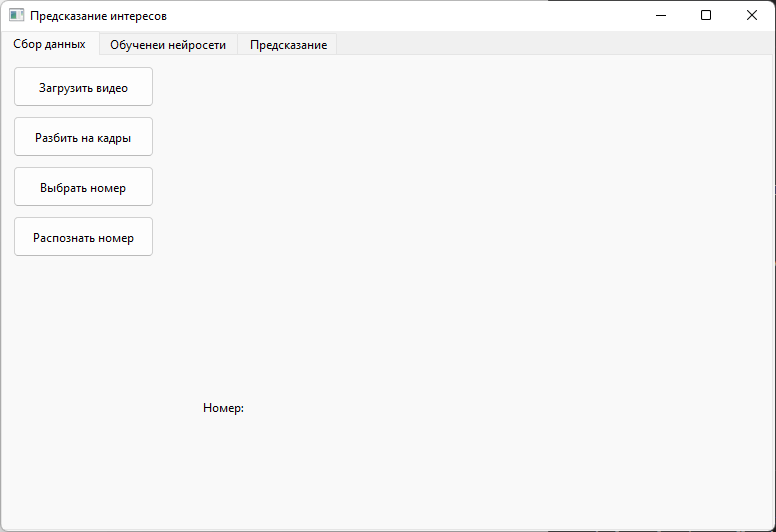
\includegraphics[width=0.5\textwidth]{window1}
	\caption{Окно программы}
	\label{f:window1}
\end{figure}

Выбор изображения представлен на рисунке~\ref{f:choose-pic}. Рядом с кнопками есть место для отрисовкм выбранного изображения.

\begin{figure}[h!]
	\centering
	\vspace{\toppaddingoffigure}
	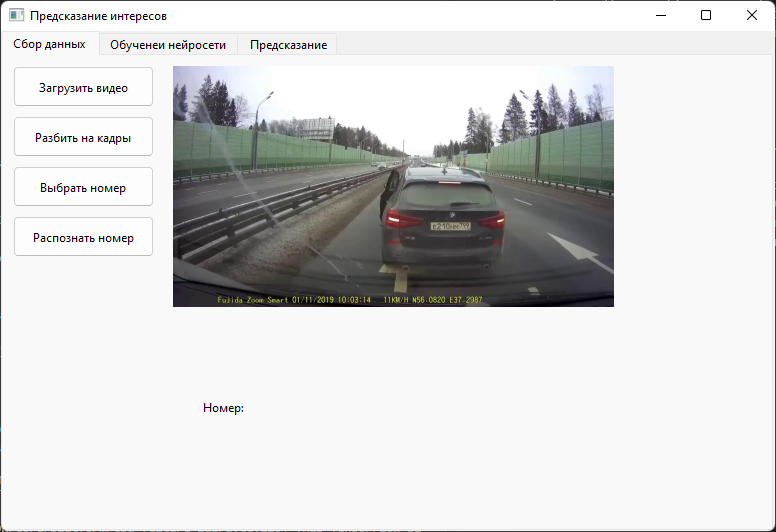
\includegraphics[width=0.5\textwidth]{choose-pic}
	\caption{Выбор изображения}
	\label{f:choose-pic}
\end{figure}

Распознавание номера представлено на рисунке~\ref{f:recognize}.

\begin{figure}[h!]
	\centering
	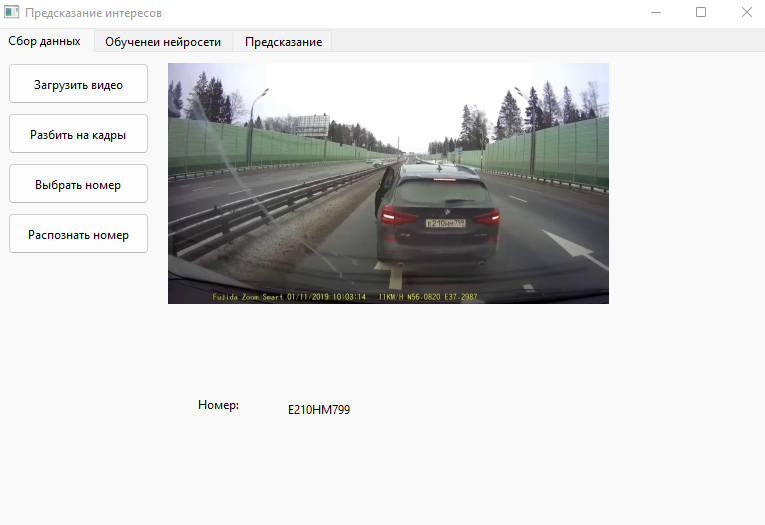
\includegraphics[width=0.5\textwidth]{recognize}
	\caption{Распознавание номера}
	\label{f:recognize}
\end{figure}


\newpage

Дальше происходит переход на сайт для определения модели автомобиля по распознанному номеру (рисунок~\ref{f:ident-model}).

\begin{figure}[h!]
	\centering
    \vspace{\toppaddingoffigure}
	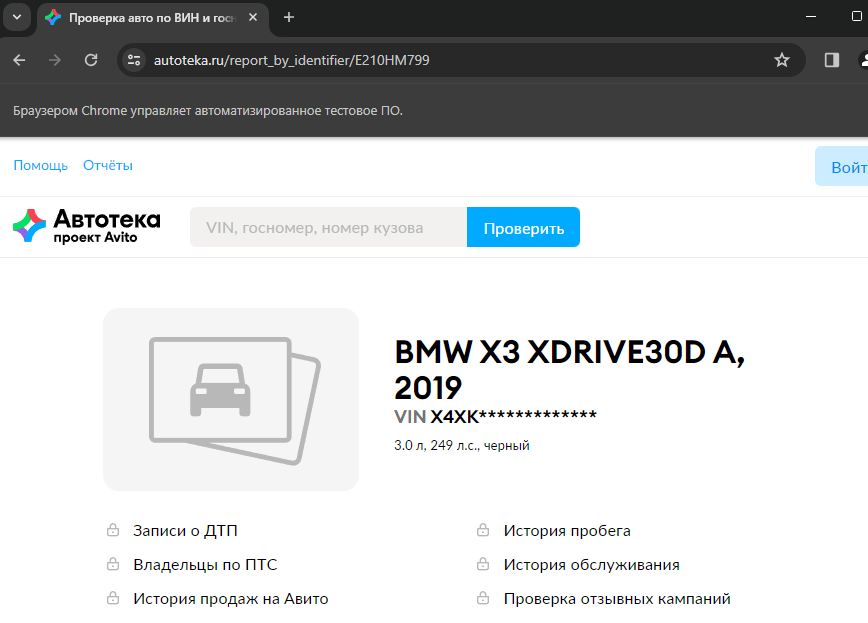
\includegraphics[width=0.5\textwidth]{ident-model}
	\caption{Определение модели авто}
	\label{f:ident-model}
\end{figure}


После этого предлагается выбрать изображение с бланком (рисунок~\ref{f:blank-examp}).

\begin{figure}[h!]
	\centering
	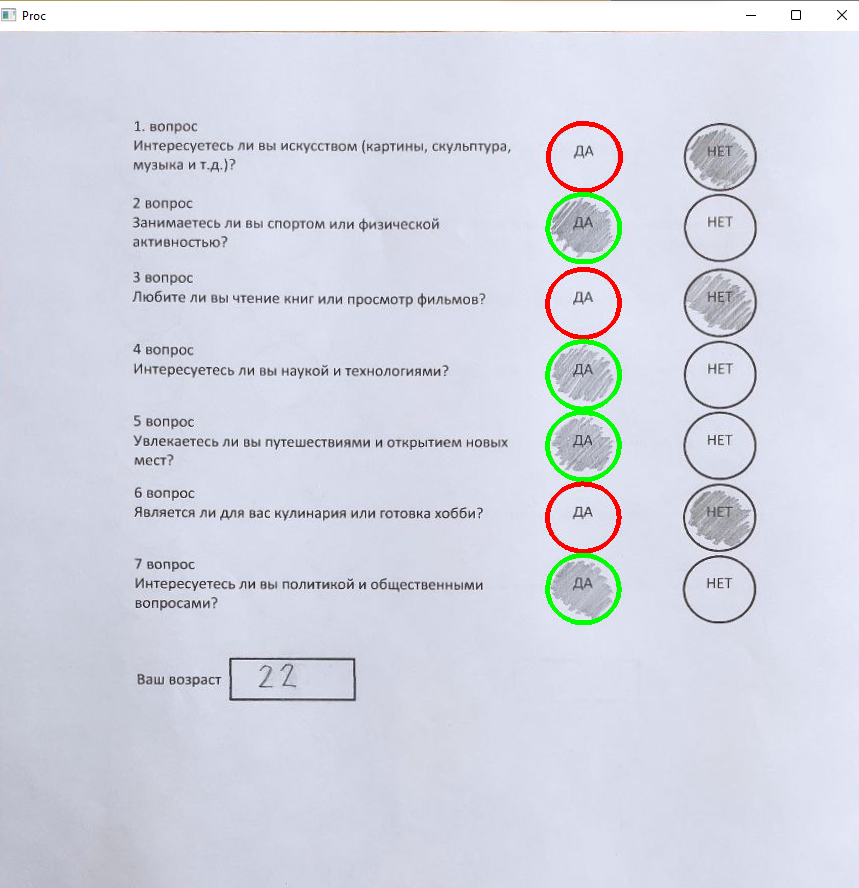
\includegraphics[width=0.5\textwidth]{blank-examp}
	\caption{Бланк опроса}
	\label{f:blank-examp}
\end{figure}


На бланке происходит обводка ответов. красным обводится в случае ответа НЕТ, а зеленым – в случае ответа ДА. Так же происходит считывание возраста, указанного в специальном поле.

Для удобства отладки происходит вывод в консоль (рисунок~\ref{f:console-log}).

\begin{figure}[h]
	\centering
	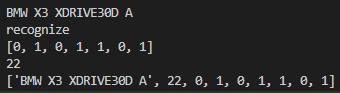
\includegraphics[width=0.5\textwidth]{console-log}
	\caption{Работа программы}
	\label{f:console-log}
\end{figure}

\newpage
Как можно увидеть по рисунку~\ref{f:console-log}, была определена модель автомобиля, так же выведен массив, содержащий ответы на вопросы. «0» означает ответ НЕТ, а «1» - ответ ДА. Кроме того, можно увидеть распознанный возраст «22». В конце все данные объединяются в единое целое, для записи в датасет – файл формата CSV. Результат записи представлен на рисунке~\ref{f:dataset}.

\begin{figure}[h!]
	\centering
    \vspace{\toppaddingoffigure}
	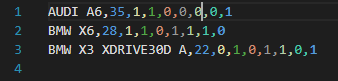
\includegraphics[width=0.5\textwidth]{dataset}
	\caption{Датасет}
	\label{f:dataset}
\end{figure}

\newpage
Окно для обучения нейросети представлено на рисунке~\ref{f:window2}. Имеются 2 кнопки дял выбора файла и начала обучения.

\begin{figure}[h!]
	\centering
    \vspace{\toppaddingoffigure}
	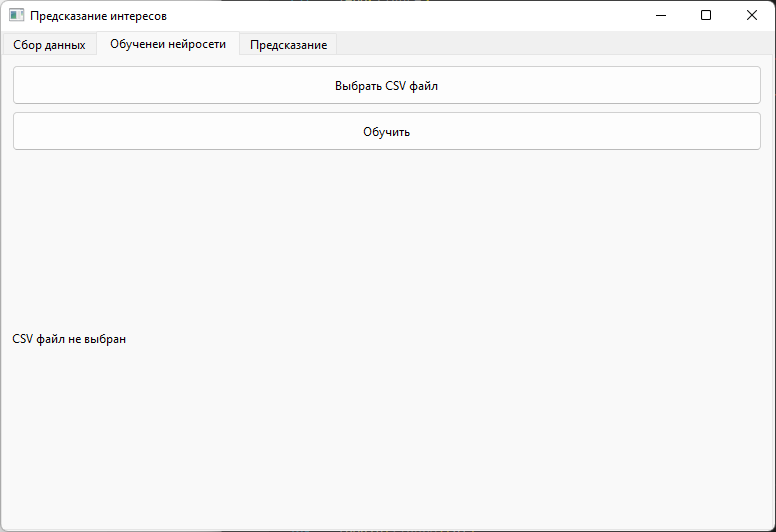
\includegraphics[width=0.5\textwidth]{window2}
	\caption{Окно программы}
	\label{f:window2}
\end{figure}

После выбора файла датасета выводится сообщение о выбранном файле (рисунок~\ref{f:window2.1}). Дальше можно приступать к обучению. По итогу обучения создается модель с расиширением ".keras".

\begin{figure}[h!]
	\centering
    \vspace{\toppaddingoffigure}
	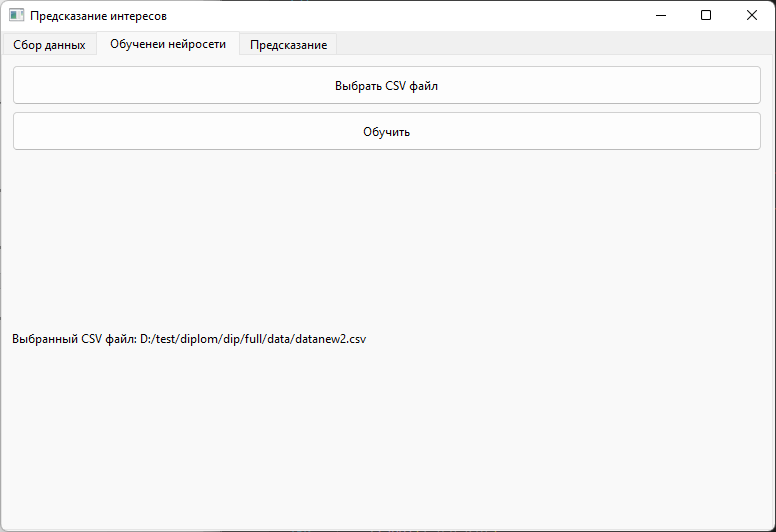
\includegraphics[width=0.5\textwidth]{window2.1}
	\caption{Окно программы}
	\label{f:window2.1}
\end{figure}

\newpage
Окно для предсказания интересов придставелно на рисунке~\ref{f:window3}.
\begin{figure}[h!]
	\centering
    \vspace{\toppaddingoffigure}
	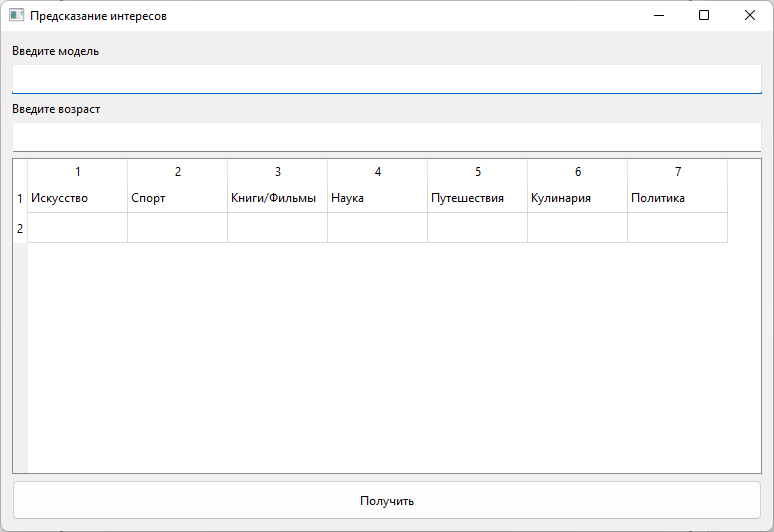
\includegraphics[width=0.5\textwidth]{window3}
	\caption{Окно программы}
	\label{f:window3}
\end{figure}

В поля для ввода необходимо ввести данные: название автомобиля и возраст владельца. После этого нажать на кнопку внизу экрана. Дальше модуль проведет работу, используя обученную модель для прогнозирования интересов. Результат работы представлен на рисунке~\ref{f:res-mod-pred}.
\begin{figure}[h!]
	\centering
    \vspace{\toppaddingoffigure}
	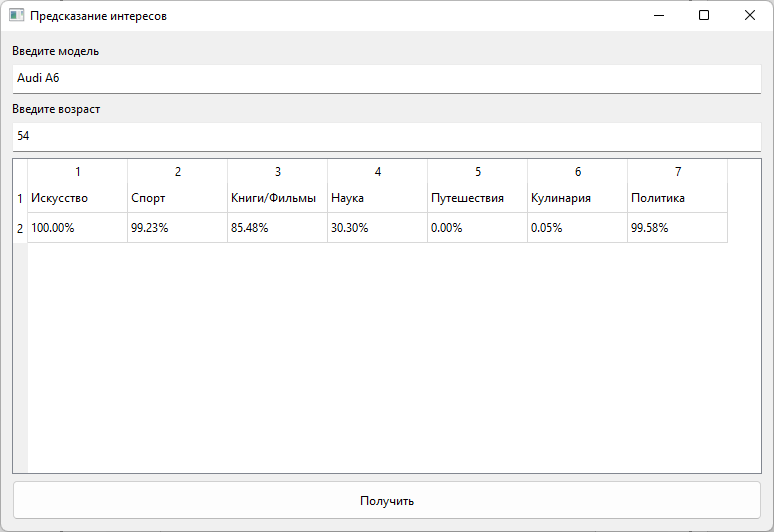
\includegraphics[width=0.5\textwidth]{res-mod-pred}
	\caption{Результат работы модуля}
	\label{f:res-mod-pred}
\end{figure}




\newpage
\section*{Выводы}
В двнном разделе были описаны основные технологии, которые использовались при разработке модулей, из которых состоит система. Было дано пояснение к основным функциям, а также расписан порядок их выполнения.